\documentclass{exam}
\usepackage{preamble}
\sisetup{group-separator = {,}}
\usepackage{exam-randomizechoices}

\def\one{123}
\def\two{2}
\def\three{3}
\def\four{4}

\def\testVersion{\one} % Edit Version number here only.

\setrandomizerseed{\testVersion}

\pagestyle{headandfoot}
\runningheadrule
\firstpageheader{Astronomy}{Semester 2 Final Exam}{May 2023}

\CorrectChoiceEmphasis{\color{red}\bfseries}
\SolutionEmphasis{\color{red}}

\printanswers

\begin{document}
\begin{questions}

\question
Identify the planet shown below.

\begin{center}
\begin{tikzpicture}[scale=0.5, transform shape]
    \clip (-0.03,0) circle (2.75cm);;
    \node at (0,0) 
        {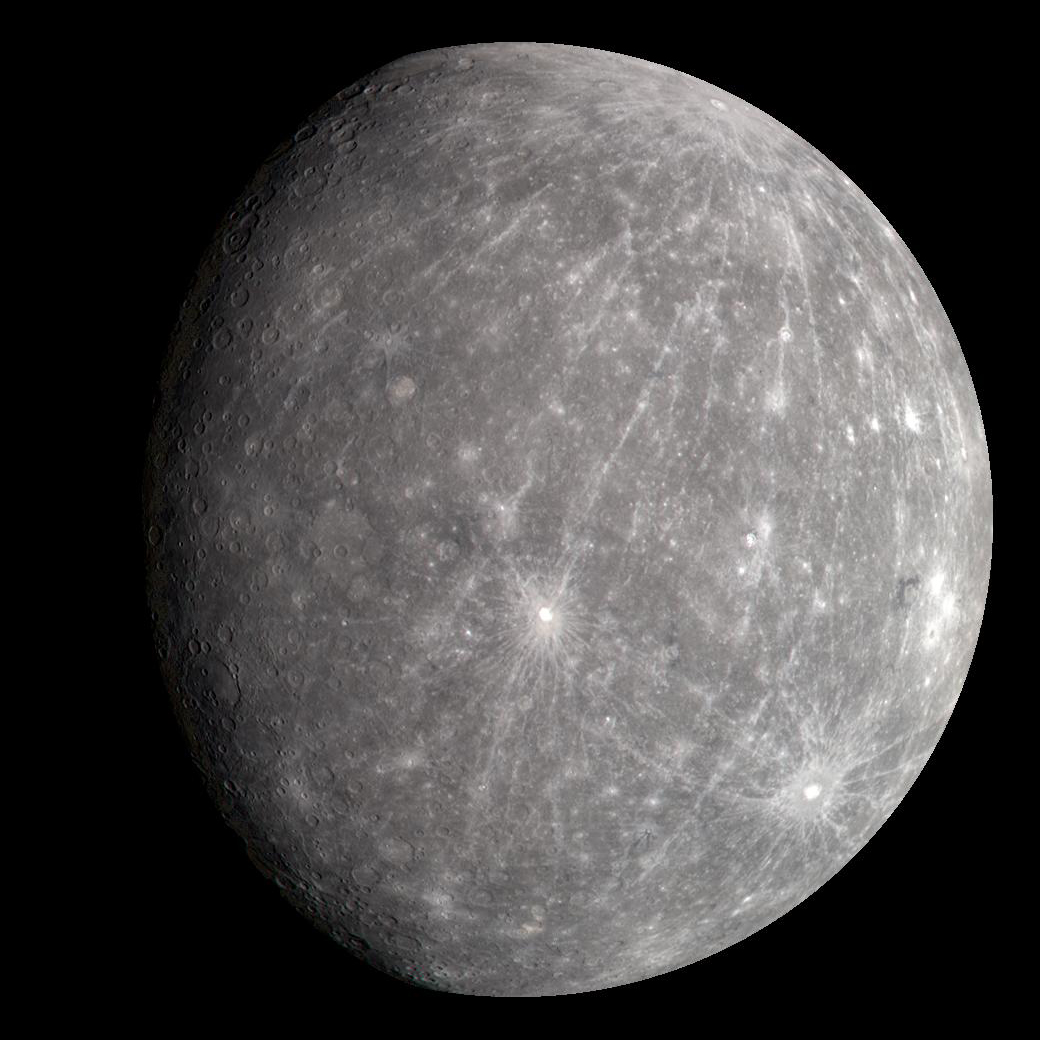
\includegraphics[width=6cm,trim={0cm 0mm 0cm 0mm}, clip]{Figures/Mercury.jpeg}};
    %\draw[red] (-0.03,0) circle (2.77cm);
    \end{tikzpicture}
\end{center}

\begin{randomizechoices}
    \correctchoice Mercury
    \choice Venus
    \choice Earth
    \choice Mars
    \choice Moon
\end{randomizechoices}

\question
Identify the planet below.

\begin{center}
\begin{tikzpicture}[scale=0.7, transform shape]
    \clip (0,0) circle (2.3cm);
    \node at (-0.02,0.08) 
        {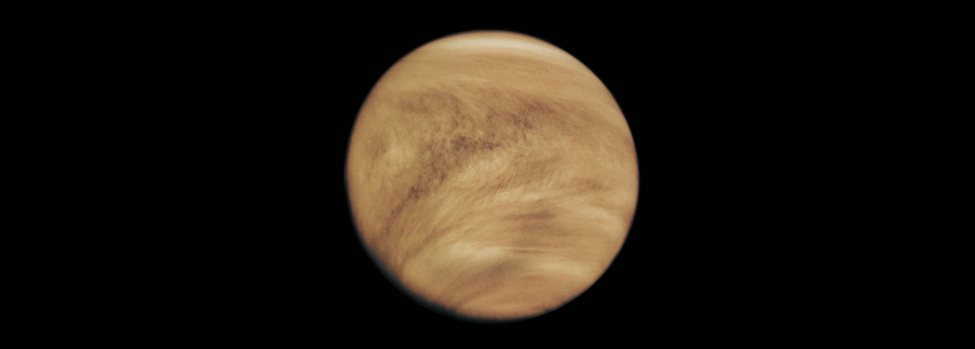
\includegraphics[width=6cm,trim={5cm 2mm 5cm 2mm}, clip]{Figures/Figure10.2.jpeg}};
    \end{tikzpicture}
\end{center}

\question
Identify the planet below.

\begin{center}
\begin{tikzpicture}[scale=0.6, transform shape]
    \clip (0,0.05) circle (2.52cm);
    \node at (-0.02,0.08) 
        {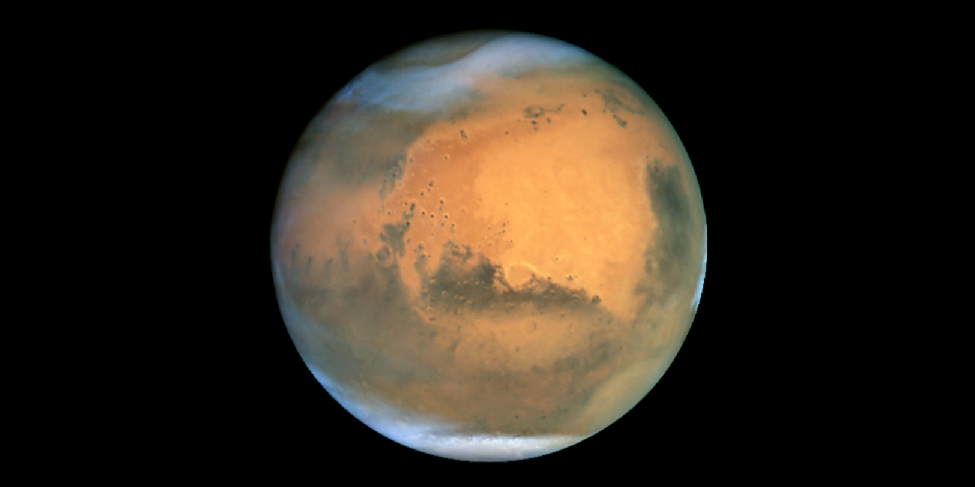
\includegraphics[width=6cm,trim={4cm 2mm 4cm 2mm}, clip]{Figures/Figure10.13.jpeg}};
    \end{tikzpicture}
\end{center}

\question
One of the terrestrial planets has thick clouds 50 kilometers above its surface. What are these clouds primarily made of?

\begin{randomizechoices}
    \correctchoice sulfuric acid
    \choice iron oxide
    \choice water
    \choice methane
\end{randomizechoices}

\question
The solar system's largest volcano, which is on Mars, is called \fillin\ .

\begin{randomizechoices}
    \correctchoice Olympus Mons
    \choice Deimos
    \choice Phobos
    \choice Triumphant Arc
    \choice Martian Maximus
\end{randomizechoices}

\question
Consider an imaginary temperature scale called \textit{Fahrenshmeit}. Suppose that the conversion from Kelvin to degrees Fahrenshmeit is given by the following formula:

\begin{equation*}
    T_{\SI{}{\degree F}} = \frac{3}{2} \left(T_{\text{K}} - 146\right) + 61
\end{equation*}

Convert the temperature at 40 kilometers above Venus' ground from Kelvin to degrees Fahrenshmeit. Select the BEST answer.

\begin{center}
    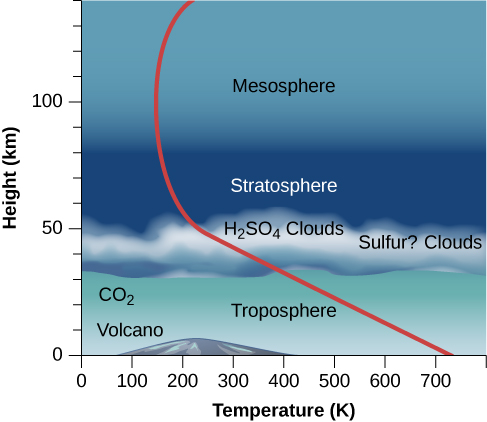
\includegraphics[width=8cm]{Figures/Figure10.12.jpeg}
\end{center}

\begin{randomizechoices}
    \correctchoice \SI{292}{\degree F}
    \choice \SI{80.3}{\degree F}
\end{randomizechoices}

\question
Identify the planet below.

\begin{center}
    \begin{tikzpicture}[scale=1, transform shape]
        \clip (0.0,0.07) circle (1.76cm);
        \node at (-0.02,0.08) 
            {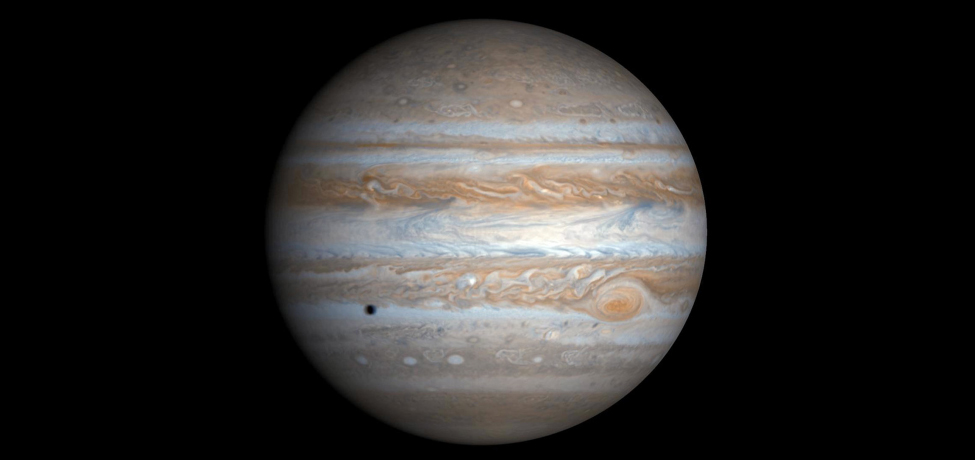
\includegraphics[width=8cm,trim={0cm 0mm 0cm 0mm}, clip]{Figures/Figure11.2.jpeg}};
            
    \end{tikzpicture}
\end{center}

\question
Identify the planet below.

\begin{center}
    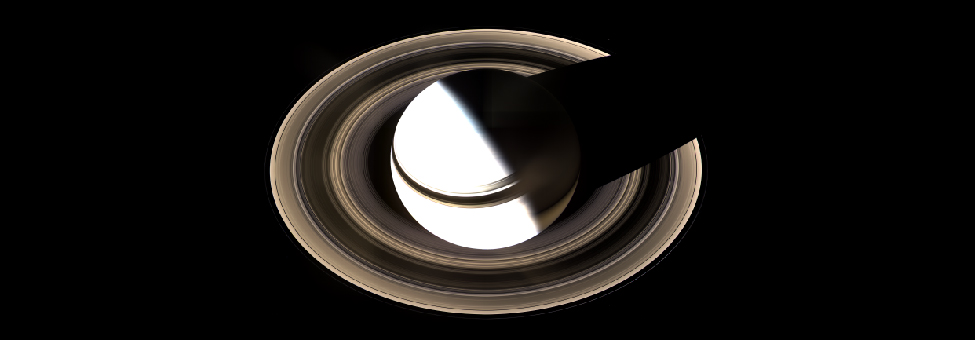
\includegraphics[width=6cm,trim={3cm 0cm 3cm 0cm},clip]{Figures/Figure7.7.jpeg}
\end{center}

\question
Identify the planet below.

\begin{center}
    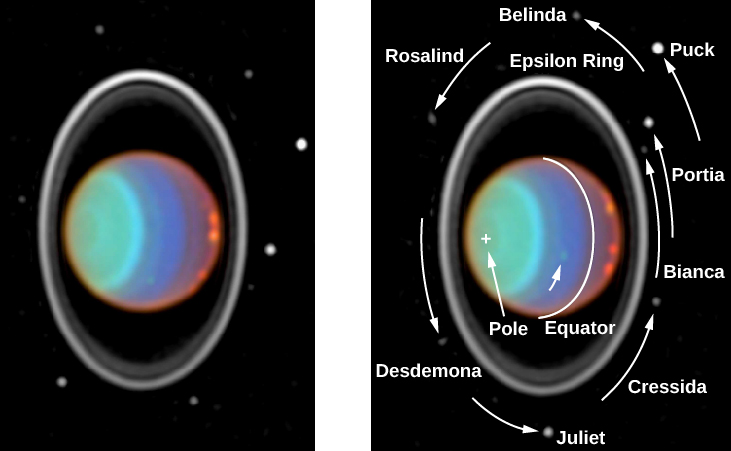
\includegraphics[width=5.5cm]{Figures/Figure11.5.jpeg}
\end{center}

\question
Identify the planet below.

\begin{center}
    \begin{tikzpicture}[scale=1, transform shape]
        \clip (0.0,-0.05) circle (1.76cm);
        \node at (0,0.0) 
            {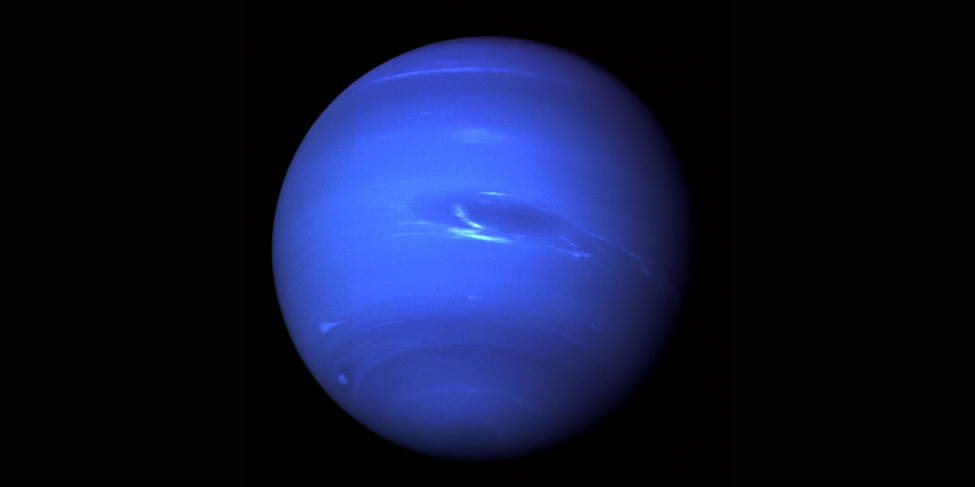
\includegraphics[width=8cm,trim={0cm 0mm 0cm 0mm}, clip]{Figures/Figure11.15.jpeg}};
    \end{tikzpicture}
\end{center}

\question
What is the distance from the Sun to Jupiter, in astronomical units?

\end{questions}
\end{document}